\documentclass[a4paper,11pt]{article}
%Przydatne paczki:
\usepackage{amssymb}
\usepackage{amsthm}
\usepackage{amsmath}
\usepackage[colorinlistoftodos]{todonotes}
\usepackage[colorlinks=true, allcolors=blue]{hyperref}
%Definicja kodowania i języka:
\usepackage[polish]{babel}
\usepackage[MeX]{polski}
\usepackage[utf8]{inputenc}
\usepackage[T1]{fontenc}
%Paczki dodane w drodze pisania:
\usepackage{graphicx}
\usepackage{anysize}
\selectlanguage{polish}
\usepackage{tabularx}
\usepackage[export]{adjustbox}
\usepackage{listings}
\usepackage{float}
\usepackage{fancyhdr}

%Nagłówek:
\pagestyle{fancy}
\fancyhead{}
\fancyhead[L]{\small{\bfseries \thepage}}
\fancyfoot[L, C, R] {}
\fancyhead[C]{\small{\bfseries Dokumentacja projektu "Reflekto"}}
\renewcommand{\headrulewidth}{0.8pt}

%\marginsize{left}{right}{top}{bottom}
\marginsize{2.5cm}{2.5cm}{2.5cm}{2.5cm}

\begin{document}

\title{Dokumentacja projektu \\ \textbf{,,Reflekto'' } }
\author{Michał Kwiecień \\ Michał Wójcik}
%skomentować żeby nie było daty
%\date{\vspace{-5ex}}
\maketitle

\begin{abstract}
Dokumentacja projektu inteligentnego lustra w konwencji IoT komunikującego się ze smartfonem z użyciem interfejsu Bluetooth Low Energy. Projekt powstał na potrzeby konkursu Nordic Semiconductor Student Contest. 
\end{abstract}

\begin{figure}
	
\includegraphics[width=0.3\textwidth,center]{logo_nordic.png}
\end{figure}

\cleardoublepage
\tableofcontents
\clearpage

\section{Ogólny opis projektu}

Założeniem projektu jest stworzenie inteligentnego lustra, które podczas wykonywania codziennych czynności, umożliwi podgląd najświeższych i spersonalizowanych informacji. Informacje te zostaną wyświetlone na ekranie umieszczonym za lustrem weneckim, dzięki czemu będą widoczne jednocześnie obok odbicia. 

Działanie lustra opiera się na przekazaniu danych poprzez moduł Bluetooth ze smartfona do modułu nRF52 i umieszczeniu ich na podłączonym ekranie. Aktywacja lustra nastąpi w momencie zbliżenia się do niego użytkownika. Z lustra może korzystać wielu użytkowników, gdyż każdorazowo przesyłane są indywidualne dane dla każdego z nich. 

W celu wygenerowania danych stworzona została dedykowana aplikacja dla systemu iOS. Po wstępnej konfiguracji umożliwi ona zautomatyzowanie procesu i przesyłanie wiadomości w tle bez późniejszych ingerencji użytkownika.


\section{Prezentacja działania}

Kiedy lustro nie jest w bliskim zasięgu jednego ze sparowanych telefonów, wyświetlana jest godzina lub pozostaje wyłączone w zależności od ustawień (Rys. \ref{lustro_off})

\begin{figure}[H]
	
\includegraphics[width=0.6\textwidth,center]{mirror_off.png}
	\caption {Lustro w stanie wyłączonym}
	\label{lustro_off}
\end{figure}

W momencie zbliżenia się użytkownika, następuje transmisja danych i wyświetlenie aktualnych wiadomości (Rys. \ref{lustro_on}).

\begin{figure}[H]
	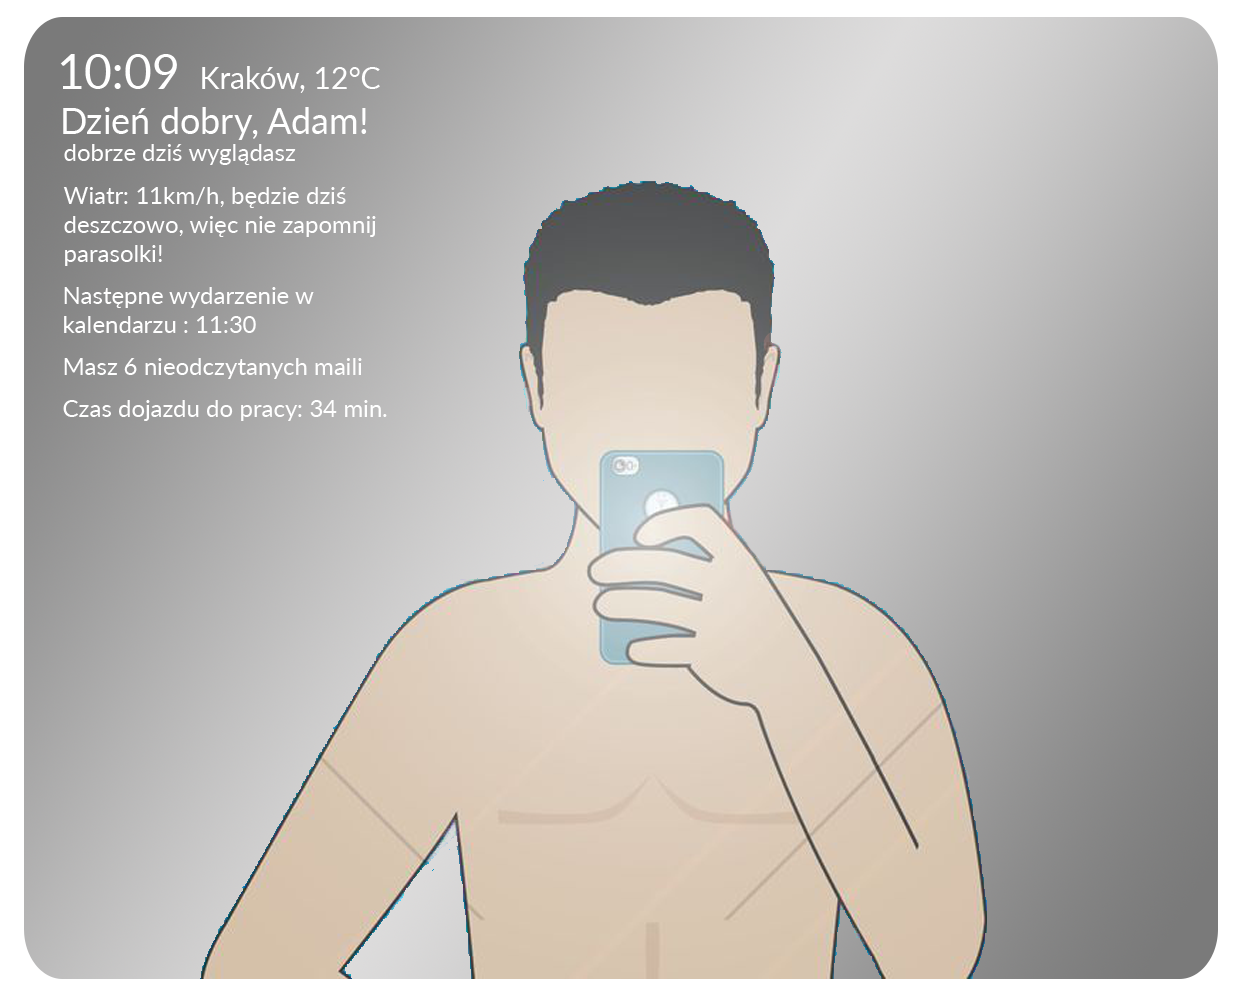
\includegraphics[width=0.6\textwidth,center]{mirror_on.png}
	\caption {Lustro w stanie aktywnym}
	\label{lustro_on}
\end{figure}

\section{Planowane możliwości personalizacji}
\begin{figure}[H]
	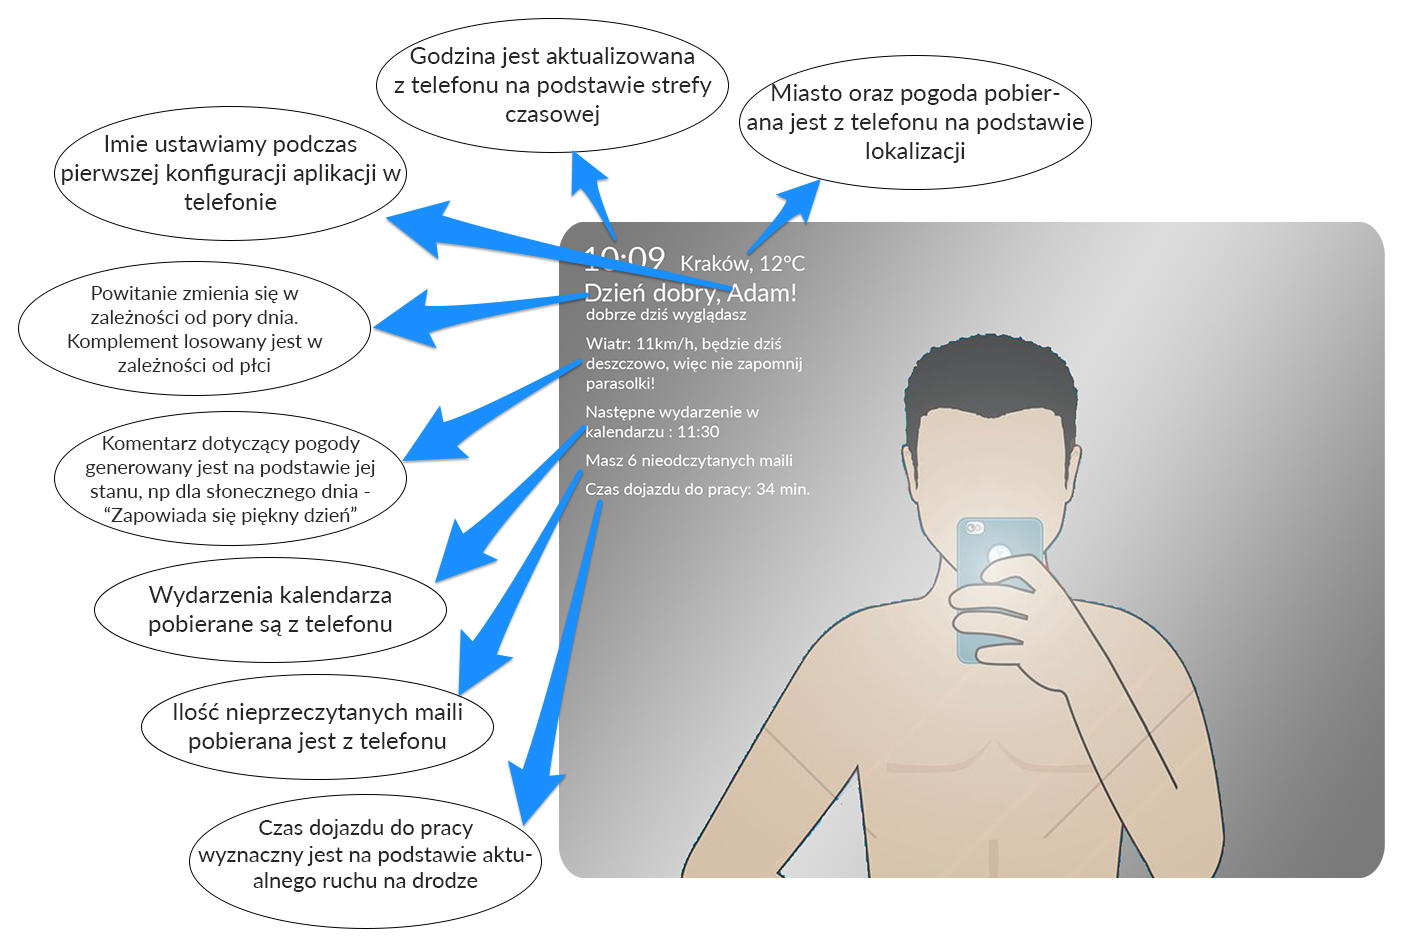
\includegraphics[width=0.9\textwidth,center]{dymki_kreski.png}
	\caption {Proponowane możlwości personalizacji}
	\label{lustro_on}
\end{figure}

\section{Opis aplikacji systemu nRF52 }

\section{Opis aplikacji systemu iOS (stan na 9 kwietnia 2017)}

Aplikacja mobilna po uruchomieniu automatycznie rozpoznaje lokalizację użytkownika z dokładnością ok. 3km oraz próbuję nawiązać połączenie bluetooth z modułem bluetooth lustra. Aktualny wygląd aplikacji pokazany jest obrazie (Rys. \ref{ios_main_screen})

\begin{figure}[H]
	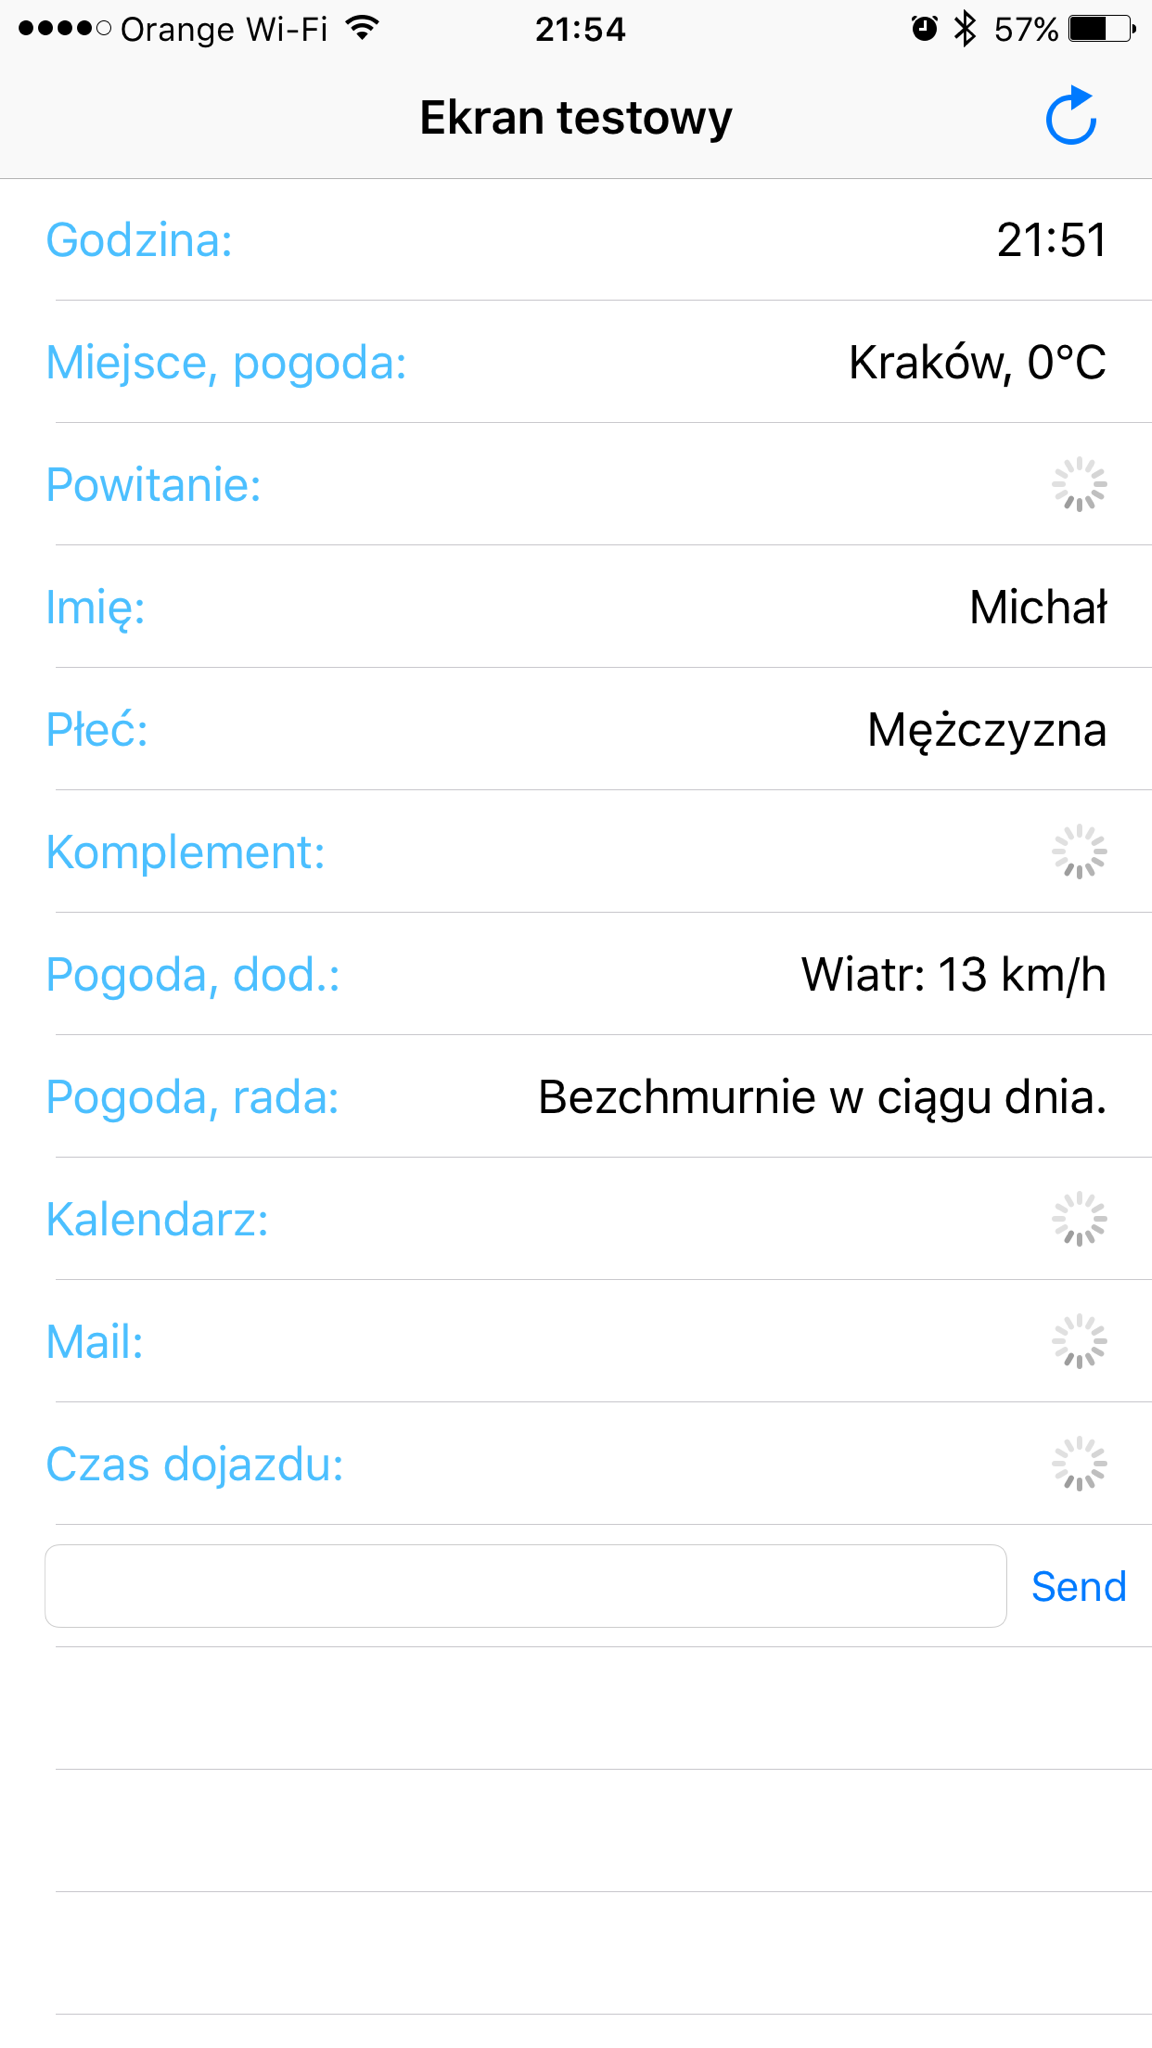
\includegraphics[width=0.5\textwidth,center]{ios_main_scrren.png}
	\caption {Aktualny wygląd aplikacji}
	\label{ios_main_screen}
\end{figure}

\subsection{Pobierane dane i sposób ich pobrania}
Aplikacja pobiera dane asynchronicznie, komórki z danymi w aplikacji uzupełniają się od razu po pobraniu poszczególnej danej. Nie trzeba czekać na zaaktualizowanie interfejsu aż do momentu pobrania każdego elementu. Poniżej opis pobierych danych oraz w przypadku bardziej złożonych danych sposób ich pozyskania.

\begin{itemize}
\item Godzina
\item Miejsce, pogoda -- na podstawie wyznaczonej lokalizacji telefon wysyła zapytanie do Dark Sky API podając w paraetrze m. in. długość oraz szerokość geograficzną. Otrzymany w odpowiedzi JSON parsowany jest na obiekt, z którego później wybierana jest temperatura. Miejsce wyznaczone jest również na podstawie szerokości i długości geograficznej używając wbudowanego  API Apple Maps.
\item Imię -- imię użytkownika rozpoznawane jest automatycznie na podstawie nazwy urządzenia. Domyślnie nazwa urządzenia to np. ,,Michal's iPhone''. W przypadku innych wersji językowych nazwa urządzenia może być inna, więc metoda wykrywająca imie może nie zadziałać. Imię, które wykryjemy będzie jedynie propozycją podczas metody konfiguracji, jeśli użytkownik stwierdzi, że nie jest to zgodne z prawdą będzie mógł je ręcznie wpisać.
\item Płeć -- wyznaczana jest na podstawie ostatniej litery imienia, również będzie możliwa zmiana podczas procesu konfiguracji.
\item Pogoda, dod. -- pobierana z Dark Sky API
\item Pogoda, rada -- pobierana z Dark Sky API
\end{itemize}

\subsection{Sposób działania}
Po dotknięciu w poszczególną komórkę zostaje wygenerowany String z dodanymi na początku dwoma bajtami, które pozwalają systemowi wbudowanemu zidentyfikować rodzaj informacji, która jest mu wysyłana. Po stworzeniu odpowiednich danych następuje próba wysłania infomarcji. Wykonywana jest na osobym wątku, aby nie blokować interfejsu użytkonika.

W dolnej części interfejsu zostało dodane pole tekstowe ułatwiające proces przygotowania systemu wbudowanego. Można dzięki niemu wpisać dowolną informację, w jego przypadku nie są dodawane dodatkowe dwa bajty na początku.

\subsection{Planowany rozwój}

Aplikacja zostanie rozbudowana o proces kofiguracji, który użytkownik będzie musiał przejść tylko za pierwszym razem. Następne uruchomienia nie będą już wymagana, aplikacja będzie działać w tle i na podstawie skanera bluetooth uruchamiać się w pobliżu lustra. Dane będą dzielone na paczki i wysyłane do modułu bluetooth lustra.

Zostaną dodane kolejne dane pobierane z urządzenia, takie jak komplement generowany na podstawie płci lub informacje o nadchodzących wydarzeniach w kalendarzu.

Dodatkowo aplikacja zostanie przepisana, tak aby używała bilioteki RxSwift, która umożliwa pisanie kodu w sposób reaktywny i funkcjonalny. Do niektórych funkcji dodane zostaną również testy jednostkowę, oraz jeśli czas na to pozwoli integracja z systemem Travis w celu zastosowania continous integration.
	
\end{document}